
\chapter{小世界网络及影响力传播基础}
在本章中,首先介绍Kleinberg小世界网络模型和影响力传播模型,然后基于影响力传播模型介绍影响力最大化算法的相关工作。最后介绍如何用蒙特卡罗模拟估算影响力大小。

\section{Kleinberg小世界模型}
Kleinberg的小世界模型是一个由$n$个节点的集合$V$生成的随机图。
$n$个节点分布在一个$\sqrt{n} \times \sqrt{n}$的二维网格上\cite{Kleinberg2000small},为了方便,
我们把网格的上边界和下边界连接起来,同时也把网格的左边界和右边界连接起来。
这样二维网格就变成了“环面”,网格中每个节点的位置都是对称的。
网格上两个节点$u$和$v$之间的曼哈顿距离(Manhattan distance)$|uv|$是
在网格上$u$到$v$的最短路径的长度。

这个随机图上有两种类型的边:{\it 强连接}和{\it 弱连接}。
强连接是任意两个曼哈顿距离不超过$p$的节点之间生成的无向边,这里$p \geq 1$是一个模型的常数。
弱连接指连接节点$u$和网格上可能相距较远的节点$v$之间的随机边。
每个节点$u$会有$q$条互相独立的弱连接边,$u$的第$i$条弱连接边以$v$为终点的概率
正比于$1/{|uv|}^\alpha$,$\alpha\geq 0$是小世界模型的参数。
我们用$1/{|uv|}^\alpha$乘以归一化因子$\mathcal{Z} = 1/\sum_{v\in V}|uv|^{-\alpha}$(在环形网格上,这个值对于任意的节点 $u\in V$都相等),这样就得到了弱连接的概率分布函数。
最初Kleinberg描述的网络模型\cite{Kleinberg2000small}中,$u$到$v$之间的弱连接被认为是有向边,这样的网络被称为{\it 有向Kleinberg小世界网络模型}。
而有些研究工作\cite{Ghasemiesfeh2013complex}中弱连接被认为是无向的,这样的网络被称为{\it 无向Kleinberg小世界网络模型}。
两个模型在本文中都被讨论了,在分析复杂传染病的传播时,我们为了和以前的工作保持一致,
采用无向Kleinberg小世界网络模型。
分析复杂传染病的路由时,我们使用有向Kleinberg小世界网络模型。

\section{影响力传播模型}
社交网络被定义为一个有向图$G=(V,E)$,其中$V$是所有节点的集合,代表着网络中的个体,$E\subseteq V \times V$是有向边的集合。
$E$是网络中的关注或者粉丝关系,每条边也会有权值,权值代表着两个人的关系密切程度或者影响程度。
因为$G$是有向图,对于一个节点$v$,我们用$N^+(v)$表示所有$v$指向的节点集合,用$N^-(v)$表示所有指向$v$的节点集合,也就是$v$的出邻居(out-neighbours)和入邻居(in-neighbours)集合。
网络中的节点都有两种状态:{\it 未激活}(inactive)和{\it 激活}(activated)。
节点可以从未感染状态转变为感染状态,但是不能反方向转变,例如不能从已感染的状态变成未感染状态。
传播的过程可以用离散的时间步骤$0,1,2,\ldots$来描述。
在社交网络模型下,影响力传播被定义为一些疾病、信息或者想法在社交网络中沿着用户之间的有向边进行扩散。
对于一次传播过程,初始状态节点都是未激活的,选定图中的一些节点,把他们的状态设定为激活。
然后每一个时间片,按照设定的传播模型逐渐去尝试激活图未激活中的节点。
如果当前时间片没有新的节点被激活为止,传播过程结束。
接下来本文介绍常见的影响力传播模型。


\subsection{独立级联模型}
\begin{figure}[h]
	\centering
	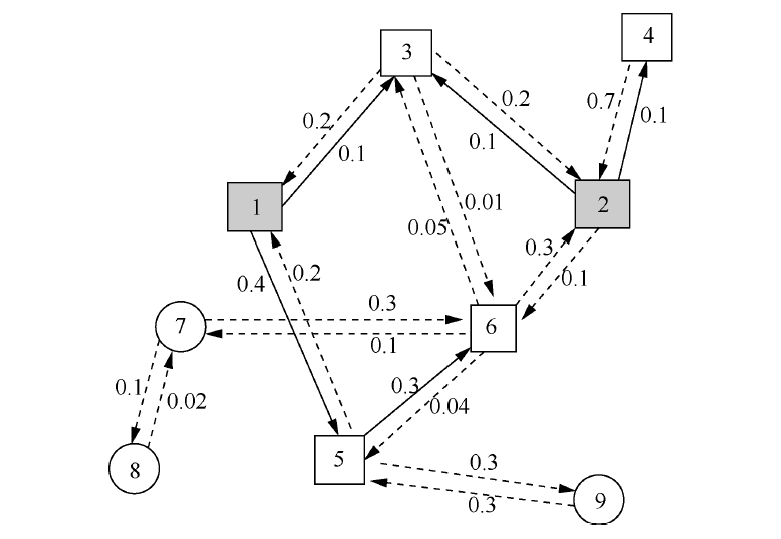
\includegraphics[width=\textwidth]{independent_cascade.png}
	\caption{独立级联模型示意}\label{fig:independent_cascade}
\end{figure}
独立级联模型(Independent Cascade Model)在03年被Kempe等人\cite{Kempe2003maximizing}提出,
在独立级联模型中,每条有向边$(u,v) \in E$都有一个概率值$p(u,v) \in [0,1]$代表着$v$被$u$影响的概率。
传播是随着离散时间片$t$增加而扩散的,定义$S_t$为到时间片$t$时刻为止被激活的节点的集合,定义$S_{-1}=\emptyset$。
在$t=0$时刻,选定$k$个节点$S_0$作为种子并把他们置为激活状态。
对于任意的$t\geq 1$时刻,每一个在$t-1$时刻激活的节点$v \in S_{t-1} \setminus S_{t-2}$都会对其所指向的未激活节点
$u \in N^+(u) \setminus S_{t}$进行一次激活尝试,成功激活$u$的概率是$p(v,u)$,不同节点之间的激活尝试相互独立。
如果节点$u$在某次激活尝试中被激活,则$u$在$t$时刻被激活。
如果$S_{t-1} \setminus S_{t-2}$中所有节点对$u$的尝试都失败,则$u$在$t$时刻未被激活。
当某一时刻没有节点被激活时,传播终止。

图\ref{fig:independent_cascade}给出了独立级联模型下的一次传播过程,图中的虚线边表示一次失败的激活尝试,实线表示成功的激活尝试。
在$t=0$时刻节点1和节点2被选为种子,在$t=1$的时刻,节点1和节点2成功激活了节点3、4、5,节点2对节点6的激活尝试失败。
在$t=2$时刻节点5成功激活了节点6,节点3和4发出的尝试激活失败。
在$t=3$时刻节点6没有激活任何节点,传播过程终止,最后被影响的节点集合是$\{1,2,3,4,5,6\}$。

\subsection{线性阈值模型}
独立级联模型(Linear Threshold Model)\cite{Kempe2003maximizing}描述的传播过程中,节点对节点的作用是互相独立的,而且每个节点只需要一次成功的激活尝试就能被激活。
而在有些场景中,一个节点的激活需要多个节点的共同作用,像购物或者接受新商品等。
为了描述类似举要多个节点累计作用才能激活的场景,线性阈值模型被提出来。

在现行与之模型中,每条有向边$(u,v) \in E$都被赋予了一个权重$w(u,v)$,对于每个节点来说,所有指向它的边权重之和不超过$1$。
也就是$\sum_{u \in N^-(u)} w(u,v) \leq 1$。
每个节点$v$还有自己的阈值$\theta_v \in [0,1]$,在传播开始前,每个节点独立的在$[0,1]$中依据均匀分布选择自己的阈值。
在每个时间节点$t \geq 1$,对于所有还没被激活的节点$v \in V \setminus S_{t-1}$,
如果由已激活节点发出的指向$v$的的有向边权重之和大于$v$的阈值,也就是$\sum_{u \in N^-(u) \cap S_{t-1}} w(u,v) \geq \theta_v$,
则$v$会在$t$时刻被激活,否则停留在未激活状态。
同样,当在某一时刻没有新节点被激活时,传播停止。

\subsection{通用级联模型}
独立级联模型的假设过强,于是Kempe\cite{Kempe2003maximizing}提出了通用级联模型(General Cascade Model),
这是独立级联模型的一般形式。
对于通用级联模型,每个节点$v$有个激活函数$p_v(u,S):N^-(v) \times 2^{N^-(v)} \to [0,1]$,
这里$S \subset N^-(v)$并且$u \in N^-(v) \setminus S$。
传播过程整体和独立级联模型一致,
在$t=0$时刻选定种子节点后,在$t \geq 1$的时间片,
对于尚未激活的节点$v \not\in S_{t-1}$,把$v$刚刚激活的的入邻居$N^-(v) \cap (S_{t-1}\setminus S_{t-2})$按照$u_1,u_2,\dots,u_{\ell}$排列,
依据这个顺序依次尝试激活节点$v$。
如果$u_1,u_2,\dots,u_{i-1}$没有成功激活$v$,则令$S = (N^-(v) \cap S_{t-2}) \cup \{u_1,u_2,\dots,u_{i-1}\}$
然后$u_{i}$以$p_v(u_i,S)$的概率尝试激活$v$。
在通用级联模型中,$p_v(u,S)$满足顺序无关性质,也就是最终$u_1,u_2,\dots,u_{\ell}$尝试激活$v$之后$v$被激活的概率
与这$\ell$次尝试的顺序无关,只与尝试激活的节点集合有关。
注意到独立级联模型是通用级联模型的特例,只需要令$p_v(u,S)$恒等于$p(u,v)$即可。


\subsection{通用阈值模型}
在通用阈值模型中(General Threshold Model),每个节点$v$有一个阈值函数$f_v:2^{N^-(v)} \to [0,1]$。
阈值函数$f_v$是单调非减(monotone)而且$f_v(\emptyset)=0$。
和线性阈值模型相同,在传播开始前,每个节点独立的在$[0,1]$中依据均匀分布选择自己的阈值。
然后在接下来的每一时刻$t\geq 1$,对于$v \not\in S_{t-1}$,
如果$f_v(S_{t-1} \cap N^-(v)) \geq \theta_v$,
节点$v$被激活,否则节点$v$保持未激活状态。

%线性阈值模型是通用阈值模型的特例,只需要令$f_v(S) = \sum_{u\in S}w(u,v)$。
通用阈值模型和通用级联模型也是等价的,给定阈值函数$f_v$,可以得到激活函数
$p_v(u,S) = \frac{f_v(S \cup \{u\}) - f_v(S)}{1-f_v(S)}$。
给定激活函数$p_v$,同样可以得到对应的通用阈值模型的阈值函数
$f_v(S) = 1 - \Pi_{i=1}^{\ell}(1-p_v(u_i, \{u_1,u_2,\dots,u_{i-1}\}))$。


\section{影响力最大化问题}
在一个$n$个节点的图中,给定影响力传播模型,最多经过$n-1$步,传播就会结束。
我们称以$S_0$为种子集合最终传播停止时被影响的节点集合是$\Phi(S_0)$。
$\Phi(S_0)$是一个依赖于影响力传播过程的随机集合。
影响力最大化问题就是在给定种子数量选择合适的种子集合的情况下最大化$\Phi(S_0)$的期望大小。
我们定义$\sigma(S_0) = \mathbb{E}(\Phi(S_0))$,$\sigma(\cdot)$就被称作为{\it 影响力函数}。
通常所研究的种子集合大小不超过$k$的影响力最大化问题可以公式化为$S^* = \mathrm{argmax}_{S \in V, |S|=k} \sigma(S)$,
$S^*$为最优解集合。
通常选用的影响力模型是独立级联模型或者线性阈值模型,近些年来也有很多基于这两个传播模型的影响力最大化算法被提出。

影响力最大化本质上描述了社交网络中的营销(Social marketing)问题,
有新的产品或者广告发布时,希望选择人试用并转发消息,然后口口相传最后扩散到很多人。
商家最后的目的就是希望可以遭到影响力最大的用户集合使得最终扩散的范围最大,这也就是影响力最大化的目标。
影响力最大化问题是社交网络中营销问题的抽象,研究影响力最大化问题对于商家试用品和广告的投放有很大帮助。
下面介绍一下影响力最大化问题的常见算法。

\subsection{贪心算法}
影响力最大化问题的复杂度很高,至少比集合覆盖最大化(Max Set Cover)问题要难,而集合覆盖最大化问题是NP-Hard的。
但是影响力函数$\sigma(\cdot)$在独立级联模型和线性阈值模型下被证明是次模的\cite{Kempe2003maximizing}。
次模函数是定义在集合函数上的,对于一个集合函数$f:2^V \to \mathbb{R}$,
如果对于任意的输入集合$S \subseteq T \subseteq V$和元素$u \in V \setminus T$都有
$f(S \cup \{u\}) - f(S) \geq f(T \cup \{u\}) - f(T)$,
则称函数$f$满足次模(submodular)性质。
次模性质本质上是边际效益递减,同样加入一个元素$u$,$f(T)$函数值的提升不如$f(S)$的提升大。
如果对于输入$S \subseteq T \subseteq V$,$f$函数还满足$f(S) \leq f(T)$,则称函数$f$是单调非减的。
对于单调非减和次模的函数$f$,贪心算法可以做到$1-\frac{1}{e}$的近似比。

\begin{algorithm}
	\caption{Maximize Monotone and Submodular Function}
	\label{alg:1} 
	\begin{algorithmic}[1]
		\REQUIRE monotone and submodular function $f:2^V \to \mathbb{R}$.
		\ENSURE $S \ subseteq V$ that achieve $1-\frac{1}{e}$ approximation-ratio.
		\STATE Initialize $N List$, each $List$ correspondences to a region in $S_{property}$;
		\STATE $R_I = \{\}$
		\FORALL {$q_I^{(k)}$ in $Q_I$}
		\STATE $index=$ the region that $q_I^{(k)}$ belongs to.
		\STATE put $q_I^{(k)}$ into $List[index]$.
		\ENDFOR
		\FORALL {$q_I^{(k)}$ in $Q_I$}
		\FOR {$i=0$ to $N-1$}
		\IF {$List[i]$ on the axes}
		\STATE re-count the points in $List[i]$.
		\ENDIF
		\ENDFOR
		\STATE update $R_I[k]$
		\ENDFOR
	\end{algorithmic} 
\end{algorithm}





\section{最新工作与研究趋势}
由于基于BoW的图像检索框架本身的特点,几何校验一直是人们研究的热点。无论是检索时检验还是检索后校验,最近几年都有更快、精度更高的方法被提出来。通过对上一节的分析我们可以看到在BoW框架下,几何校验存在两个固有难题:一个是会显著增加计算复杂度;另一个是无法很好的解决图片旋转的问题。例如基于RANSAC的方法\cite{philbin2007object}\cite{chum2007total}只能对TopN的图片进行校验,并且需要重力向量假设(即图片不存在旋转);同样WGC和SPM都无法解决图片旋转的问题,并且需要额外的计算和存储资源。所以目前的在BoW框架下的研究趋势是:
\begin{enumerate}
	\item 快速的几何校验;
	\item 尽可能减少内存;
	\item 全局几何校验与局部几何校验结合;
	\item 检索时校验与检索后校验结合;
\end{enumerate}

在最新的几何校验算法中,\cite{Zhong2015Fast}对FSM进行了改进,提出了更快的后校验方案DSM;\cite{li2015pairwise}提出了pair-wise的几何校验,结合图像全局的几何关系和特征点局部的几何关系,得到了state-of-the-art的检索精度。

由于基于CNN的图像检索框架提取的图片的全局特征,不存在局部特征之间的几何校验问题,即图片的几何关系已经编码到了全局特征中了。但是,基于CNN的检索框架并没有很好的解决图片旋转的问题,目前对于查询图片存在旋转的情况主要通过以下方法进行处理:
\begin{enumerate}
	\item 人为的将图片调整为竖直方向\cite{babenko2014neural},这种方法不适用于实际的系统;
	\item 在训练时进行数据扩大,即把图片各个方向的版本都输入的CNN中参与训练\cite{babenko2014neural},这种方法会延长训练时间;
	\item 通过Max Pooling的手段,将不同角度的图片的全局特征融合为一个全局特征\cite{chandrasekhar2015practical},这种方法不具有扩展性。
\end{enumerate}


\section{本文的研究框架与思路}
\begin{figure}[h]
	\centering
	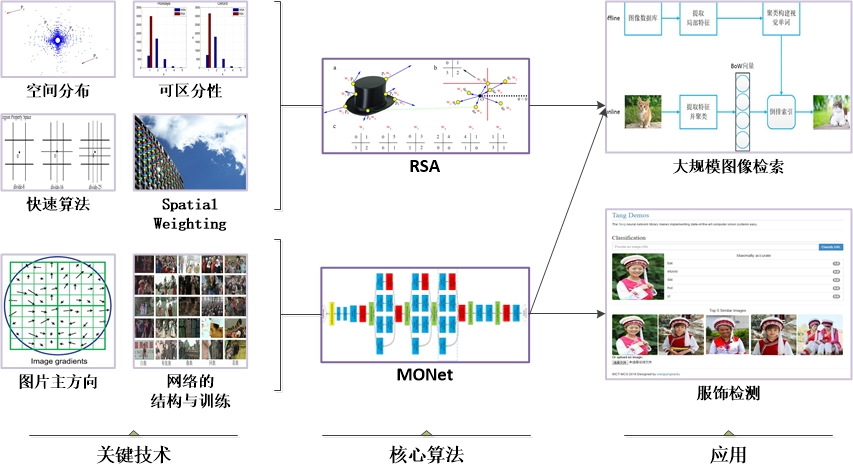
\includegraphics[width=0.9\textwidth]{frame_3.jpg}
	\caption{研究框架图}\label{fig:frame}
\end{figure}
尽管研究者们已经对图像检索中的几何校验做出了各种各样的尝试,但该领域仍然存在许多尚待解决的问题。例如如何快速的进行几何校验,同时不增加系统的负担;如何更好的解决图片旋转的问题,使几何校验算法可以更好的应用于实际的图像检索系统中去。为了解决上述问题,本文按照图\ref{fig:frame}所示的框架,提出了更加实用的几何校验方案Region Similarity Arrangement(RSA)。RSA不会增加BoW检索框架的内存,并且只需要很少的计算量,但是可以显著的提高的BoW baseline的检索精度。同时利用了CNN可以更好的理解图片语义信息这一特点,提出了Main Orientation Net(NMOet)。MONet不仅可以对基于CNN的图像检索框架提供一定的几何校验,同时可以应用于传统的BoW框架中,解决了传统几何校验方案无法处理图片旋转的问题。

\section{本章小结}
本章介绍了基于BoW和基于CNN的图像检索框架。基于BoW的图像检索已经是一种比较成熟的框架,已经存在很多经典的改进算法,本章对这些算法也进行了详细的介绍,包括查询扩充、软量化、注入技术和RootSIFT。对于BoW图像检索中的几何校验算法,本章介绍了三种经典的算法,包括两种后校验算法FSM和WGC和一种检索时算法SPM。对于以上算法,我们对其优劣进行了简单的分析和总结。另外,本章还介绍了国际上关于该课题最新的一些思路和研究趋势,这为我们未来的工作指明了方向。在本章的最后,我们提出了自己的研究框架与思路,在接下来的章节中,我们将按照该框架展开我们的研究工作。

